\documentclass[12pt,a4paper]{article}

\usepackage[utf8]{inputenc}
\usepackage[T1]{fontenc}
\usepackage[brazilian]{babel}
\usepackage{lmodern}
\usepackage{geometry}
\usepackage{graphicx}
\usepackage{booktabs}
\usepackage{array}
\usepackage{float}
\usepackage{xcolor}
\usepackage{amsmath}
\usepackage{listings}
\usepackage{hyperref}
\usepackage{fancyhdr}
\usepackage{microtype}

\geometry{top=2.3cm,bottom=2.3cm,left=2.5cm,right=2.5cm}
\graphicspath{{prints/}}
\hypersetup{colorlinks=true,linkcolor=blue!45!black,urlcolor=blue!55!black}

\pagestyle{fancy}
\fancyhf{}
\lhead{Automação Inteligente}
\rhead{Atividade Prática 3A}
\cfoot{\thepage}
\setlength{\headheight}{15pt}

\definecolor{codebg}{RGB}{246,248,250}
\definecolor{codegreen}{RGB}{24,120,70}
\definecolor{codeblue}{RGB}{30,70,170}

\lstdefinelanguage{Scilab}{
  morekeywords={if,then,elseif,else,end,for,while,try,catch,function,return,clear,clc},
  sensitive=true,
  morecomment=[l]{//},
  morestring=[b]"
}

\lstset{
  language=Scilab,
  basicstyle=\ttfamily\fontsize{7}{8}\selectfont,
  keywordstyle=\color{codeblue}\bfseries,
  commentstyle=\color{codegreen},
  stringstyle=\color{orange!60!black},
  backgroundcolor=\color{codebg},
  frame=single,
  breaklines=true,
  showstringspaces=false,
  numbers=left,
  numberstyle=\tiny\color{gray},
  tabsize=4,
  literate={Ç}{{\c{C}}}1
}

\begin{document}

\hypersetup{pageanchor=false}
\begin{titlepage}
  \centering
  {\large Disciplina: Automação Inteligente\par}
  \vspace{2.2cm}
  {\Large\bfseries ATIVIDADE PRÁTICA 3A -- LÓGICA FUZZY\par}
  \vspace{0.6cm}
  {\LARGE\bfseries Controle Fuzzy para Desvio de Obstáculos em Robótica Móvel\par}
  \vspace{1.2cm}
  {\large Projeto, cálculo manual e implementação computacional de um sistema Mamdani\par}
  \vfill
  \begin{tabular}{rl}
    \textbf{Aluno:} & Fernando Roque Caldas de Oliveira \\
    \textbf{Matrícula:} & 202211130038 \\
    \textbf{Software:} & Scilab 6.1.1 (Windows 64 bits) \\
    \textbf{Módulo:} & sciFLT 0.5
  \end{tabular}
  \vfill
  {\large 2026\par}
\end{titlepage}

\hypersetup{pageanchor=true}
\pagenumbering{roman}
\tableofcontents
\newpage
\pagenumbering{arabic}

\section{Objetivo}

O objetivo desta atividade é projetar e implementar um controlador fuzzy reativo para um robô móvel. O sistema recebe a distância frontal até um obstáculo e a assimetria entre os sensores laterais. A saída é um ângulo de correção que permite desviar do obstáculo de maneira suave.

Foi utilizado um sistema Mamdani com conectivo E pelo mínimo, implicação pelo mínimo, agregação pelo máximo e defuzzificação pelo centroide. A implementação foi realizada exclusivamente no Scilab 6.1.1 para Windows, com o módulo sciFLT 0.5.

\section{Variáveis linguísticas}

\subsection{Distância frontal}

A distância frontal $d$ pertence ao universo $[0,100]$ cm e possui os termos Perto, Média e Longe.

\begin{figure}[H]
  \centering
  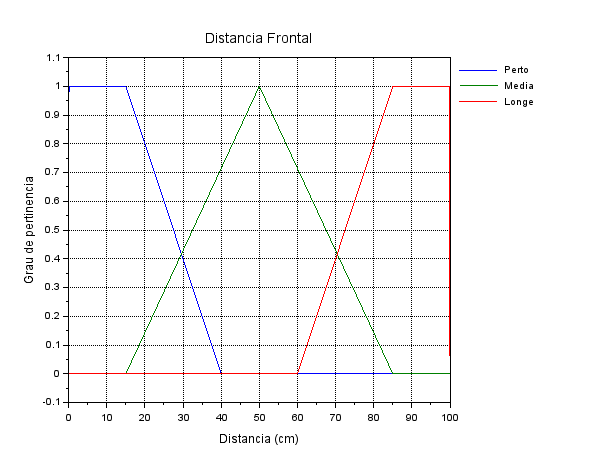
\includegraphics[width=0.82\textwidth]{01_distancia_frontal.png}
  \caption{Funções de pertinência da distância frontal.}
\end{figure}

\subsection{Assimetria lateral}

A assimetria é definida por $a=d_{dir}-d_{esq}$ e pertence ao universo $[-50,50]$ cm. Valores negativos indicam obstáculo mais próximo do lado direito. Os termos são Negativa, Zero e Positiva.

\begin{figure}[H]
  \centering
  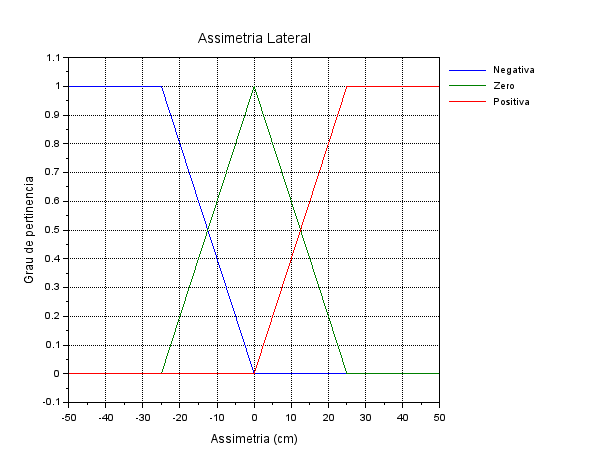
\includegraphics[width=0.82\textwidth]{02_assimetria_lateral.png}
  \caption{Funções de pertinência da assimetria lateral.}
\end{figure}

\subsection{Ângulo de direção}

O ângulo $\theta$ pertence ao universo $[-45^\circ,45^\circ]$. Valores negativos indicam giro para a esquerda e valores positivos indicam giro para a direita. Os termos são Virar à Esquerda, Seguir em Frente e Virar à Direita.

\begin{figure}[H]
  \centering
  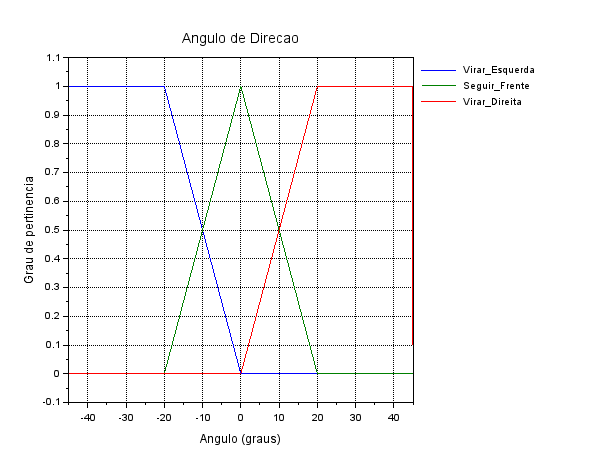
\includegraphics[width=0.82\textwidth]{03_angulo_direcao.png}
  \caption{Funções de pertinência do ângulo de direção.}
\end{figure}

\section{Base de regras}

Todas as regras utilizam o conectivo E. A base completa possui nove regras.

\begin{table}[H]
  \centering
  \caption{Base de regras do controlador fuzzy.}
  \renewcommand{\arraystretch}{1.35}
  \begin{tabular}{>{\bfseries}lccc}
    \toprule
    Distância / Assimetria & Negativa & Zero & Positiva \\
    \midrule
    Perto & Virar à esquerda & Virar à direita & Virar à direita \\
    Média & Virar à esquerda & Seguir em frente & Virar à direita \\
    Longe & Seguir em frente & Seguir em frente & Seguir em frente \\
    \bottomrule
  \end{tabular}
\end{table}

\section{Cálculo manual para \texorpdfstring{$d=10$ cm e $a=-10$ cm}{d=10 cm e a=-10 cm}}

\subsection{Fase 1 -- Fuzzificação}

Para a distância frontal, $d=10$ cm está no trecho constante da função Perto
($0\leq d\leq 15$), antes do suporte da função Média ($d<15$) e antes do
suporte da função Longe ($d<60$). Portanto:
\[
\mu_{\text{Perto}}(10)=1,
\qquad
\mu_{\text{Média}}(10)=0,
\qquad
\mu_{\text{Longe}}(10)=0.
\]

Para a assimetria lateral, $a=-10$ cm pertence simultaneamente aos trechos
lineares de Negativa e Zero. Usando as equações das retas indicadas no gráfico:
\[
\mu_{\text{Negativa}}(-10)
=\frac{0-a}{0-(-25)}
=\frac{0-(-10)}{25}
=\frac{10}{25}=0{,}4,
\]
\[
\mu_{\text{Zero}}(-10)
=\frac{a-(-25)}{0-(-25)}
=\frac{-10+25}{25}
=\frac{15}{25}=0{,}6,
\]
e $\mu_{\text{Positiva}}(-10)=0$, pois a função Positiva só possui suporte
a partir de $a=0$.

\subsection{Fase 2 -- Regras ativadas}

Somente duas regras apresentam antecedente diferente de zero:

\begin{enumerate}
  \item Se a distância é Perto e a assimetria é Negativa, então Virar à Esquerda.
  \item Se a distância é Perto e a assimetria é Zero, então Virar à Direita.
\end{enumerate}

\subsection{Fase 3 -- Conectivo E e implicação}

Pelo operador mínimo:
\[
\alpha_1=\min(1;0{,}4)=0{,}4,
\qquad
\alpha_2=\min(1;0{,}6)=0{,}6.
\]

A implicação de Mamdani trunca Virar à Esquerda em 0,4 e Virar à Direita em 0,6.

\subsection{Fase 4 -- Agregação}

As saídas truncadas são combinadas pelo máximo:
\[
\mu_{agregada}(\theta)=\max\left(
\min(0{,}4;\mu_{\text{Esquerda}}(\theta)),
\min(0{,}6;\mu_{\text{Direita}}(\theta))
\right).
\]

\subsection{Fase 5 -- Defuzzificação}

O universo de saída foi discretizado em passos de $5^\circ$, exatamente como
solicitado. Em cada ponto calcula-se primeiro
$\mu_{agregada}(\theta)$ e depois o produto
$\mu_{agregada}(\theta)\theta$.

\begin{table}[H]
\centering
\caption{Valores usados no cálculo do Centro de Área.}
\begin{tabular}{rrr@{\qquad}rrr}
\toprule
$\theta$ & $\mu$ & $\mu\theta$ & $\theta$ & $\mu$ & $\mu\theta$ \\
\midrule
-45 & 0,40 & -18,00 & 5  & 0,25 & 1,25 \\
-40 & 0,40 & -16,00 & 10 & 0,50 & 5,00 \\
-35 & 0,40 & -14,00 & 15 & 0,60 & 9,00 \\
-30 & 0,40 & -12,00 & 20 & 0,60 & 12,00 \\
-25 & 0,40 & -10,00 & 25 & 0,60 & 15,00 \\
-20 & 0,40 & -8,00  & 30 & 0,60 & 18,00 \\
-15 & 0,40 & -6,00  & 35 & 0,60 & 21,00 \\
-10 & 0,40 & -4,00  & 40 & 0,60 & 24,00 \\
-5  & 0,25 & -1,25  & 45 & 0,60 & 27,00 \\
0   & 0,00 & 0,00   &    &      &       \\
\bottomrule
\end{tabular}
\end{table}

\subsubsection*{Memorial de cálculo manual do CDA}

No lado esquerdo, existem oito amostras com pertinência $0{,}40$ entre
$-45^\circ$ e $-10^\circ$, além da amostra $-5^\circ$ com pertinência
$0{,}25$. No lado direito, as pertinências são $0{,}25$ em $5^\circ$,
$0{,}50$ em $10^\circ$ e $0{,}60$ nas sete amostras de $15^\circ$ a
$45^\circ$. Assim, o denominador do CDA é:
\begin{align*}
\sum \mu(\theta)
&=\underbrace{(8\cdot0{,}40+0{,}25)}_{3{,}45}
 +\underbrace{(0{,}25+0{,}50+7\cdot0{,}60)}_{4{,}95}\\
&=3{,}45+4{,}95=8{,}40.
\end{align*}

O numerador, incluindo os sinais dos ângulos, é:
\begin{align*}
\sum \mu(\theta)\theta
&=\underbrace{0{,}40(-45-40-35-30-25-20-15-10)
 +0{,}25(-5)}_{-89{,}25}\\
&\quad+\underbrace{0{,}25(5)+0{,}50(10)
 +0{,}60(15+20+25+30+35+40+45)}_{132{,}25}\\
&=-89{,}25+132{,}25=43{,}00.
\end{align*}

Substituindo os dois somatórios na fórmula do Centro de Área:
\[
\boxed{\theta_{manual}
=\frac{\sum \mu(\theta)\theta}{\sum \mu(\theta)}
=\frac{43{,}00}{8{,}40}
=5{,}1190^\circ}
\]

O resultado é positivo, portanto a decisão é \textbf{virar para a direita}.

\section{Implementação computacional}

O sistema foi implementado com as funções \texttt{newfls}, \texttt{addvar}, \texttt{addmf}, \texttt{addrule}, \texttt{evalfls} e \texttt{savefls} do sciFLT. A avaliação computacional utiliza 1001 pontos no universo da saída.

Para $d=10$ cm e $a=-10$ cm, o software produziu:

\begin{itemize}
  \item ângulo: $\theta=4{,}828622^\circ$;
  \item ação: virar para a direita;
  \item diferença em relação ao cálculo manual: $-0{,}290426^\circ$.
\end{itemize}

\begin{figure}[H]
  \centering
  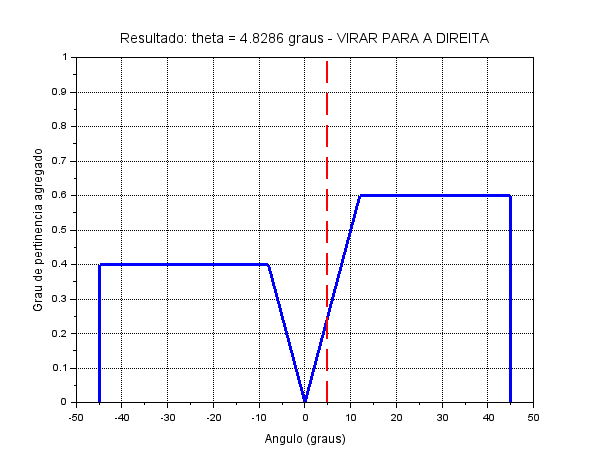
\includegraphics[width=0.9\textwidth]{resultado_simulacao.png}
  \caption{Saída agregada e ângulo defuzzificado pelo sciFLT.}
\end{figure}

A pequena diferença é esperada porque o cálculo manual utiliza passos de $5^\circ$, enquanto o programa emprega uma discretização muito mais fina.

\section{Superfície tridimensional de controle}

A Figura~\ref{fig:superficie} apresenta o mapeamento completo entre as duas entradas e o ângulo de saída. A região azul representa correções para a esquerda, a região vermelha representa correções para a direita e a região próxima de zero corresponde ao deslocamento em frente.

\begin{figure}[H]
  \centering
  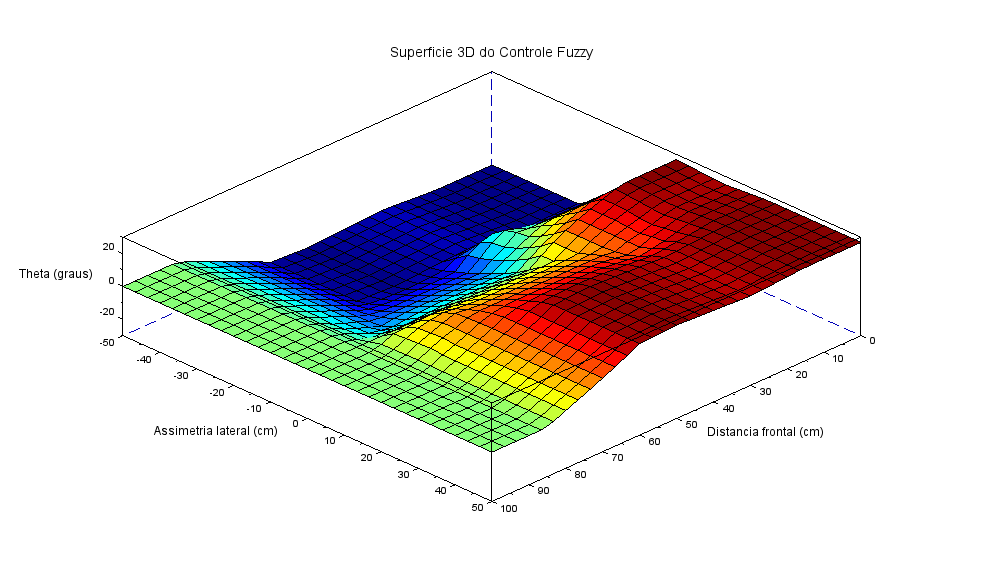
\includegraphics[width=\textwidth]{04_superficie_controle_3d.png}
  \caption{Superfície tridimensional do controlador fuzzy.}
  \label{fig:superficie}
\end{figure}

\section{Execução no Windows}

O projeto foi preparado para Windows 10 ou 11, em 64 bits, utilizando somente o Scilab 6.1.1 e o sciFLT 0.5. No console do Scilab, devem ser executados os comandos:

\begin{lstlisting}
cd("C:/Users/ferna/Desktop/01 - Faculdade/Faculdade/10 semestre/AUTOMAÇAO")
exec("fuzzy_robotica.sce", -1)
\end{lstlisting}

O código-fonte está em:
\begin{center}
\small\ttfamily
\parbox{0.95\textwidth}{\centering
C:/Users/ferna/Desktop/01 - Faculdade/Faculdade/10 semestre/\allowbreak
AUTOMA\c{C}AO/\allowbreak fuzzy\_robotica.sce}
\end{center}

O relatório, o arquivo do sistema fuzzy, o resultado numérico e os gráficos ficam na mesma pasta do projeto. As imagens são armazenadas na subpasta \texttt{prints}.

\section{Verificação dos itens solicitados}

\begin{table}[H]
\centering
\small
\caption{Conferência da entrega em relação ao enunciado da atividade.}
\renewcommand{\arraystretch}{1.25}
\begin{tabular}{>{\raggedright\arraybackslash}p{0.39\textwidth}>{\raggedright\arraybackslash}p{0.49\textwidth}}
\toprule
\textbf{Exigência} & \textbf{Atendimento} \\
\midrule
Cinco fases do cálculo manual & Seções 4.1 a 4.5, com equações, regras, implicação, agregação e CDA. \\
CDA em passos de $5^\circ$ & Tabela completa de $-45^\circ$ a $45^\circ$ e memorial dos dois somatórios. \\
Implementação computacional & Código Scilab/sciFLT, sistema salvo em \texttt{.fls} e nove regras. \\
Teste $d=10$ e $a=-10$ & Print da saída e valor computacional $4{,}828622^\circ$. \\
Comparação manual/computacional & $5{,}119048^\circ$ contra $4{,}828622^\circ$; diferença de $-0{,}290426^\circ$. \\
Documentação e GitHub & README completo, código, relatório e pasta \texttt{prints} organizados. \\
\bottomrule
\end{tabular}
\end{table}

\section{Conclusão}

O controlador fuzzy foi implementado e validado com as nove regras especificadas. Para as entradas solicitadas, tanto o cálculo manual quanto a simulação computacional indicam giro para a direita. A diferença numérica é pequena e decorre exclusivamente da resolução usada na defuzzificação. A superfície tridimensional confirma transições suaves entre as ações de virar à esquerda, seguir em frente e virar à direita.

\clearpage
\appendix
\section{Código-fonte completo em Scilab}

\lstinputlisting{fuzzy_robotica.sce}

\end{document}
